\documentclass[conference]{IEEEtran}

\IEEEoverridecommandlockouts %To add sponsors and index terms

\usepackage{cite}

\ifCLASSINFOpdf
   \usepackage[pdftex]{graphicx}
  % declare the path(s) where your graphic files are
   \graphicspath{{../images/}}
  % and their extensions so you won't have to specify these with
  % every instance of \includegraphics
   \DeclareGraphicsExtensions{.pdf,.jpeg,.png}
\else
\fi

\usepackage[cmex10]{amsmath}
%\usepackage[hidelinks]{hyperref}
\usepackage{nohyperref}
\usepackage{url}
%for columns spanning multiple rows in tables
\usepackage{multirow}
%use the booktabs package to get (much!) better vertical spacing above and below "rules" (horizontal lines), resulting in a much more professional look of your tables.
%use the colortbl package to add color to tables.
\usepackage{booktabs,colortbl}

\usepackage{amsfonts}

% correct bad hyphenation here
\hyphenation{op-tical net-works semi-conduc-tor}

  \renewcommand\footnoterule{\vspace*{-3pt}%
     \hrule width 2in height 0.4pt
     \vspace*{2.6pt}}

\begin{document}
%
% paper title
% can use linebreaks \\ within to get better formatting as desired
\title{Temperature-based Instanton Analysis: \\
Identifying Vulnerability in Transmission Networks}


% author names and affiliations
% use a multiple column layout for up to two different
% affiliations
\author{%

\IEEEauthorblockN{Jonas Kersulis,\\ Ian Hiskens}
%\IEEEauthorblockA{Electrical Engineering and Computer Science\\
\IEEEauthorblockA{Elec. Eng. and Computer Science \\
University of Michigan\\
Ann Arbor, MI, United States\\}
\and
\IEEEauthorblockN{Michael Chertkov,\\Scott Backhaus}
%\IEEEauthorblockA{Center for Nonlinear Studies\\
\IEEEauthorblockA{Center for Nonlinear Studies\\
Los Alamos National Laboratory\\
Los Alamos, NM, United States\\
}
\and
\IEEEauthorblockN{Daniel Bienstock\\ \hspace{1pt} }
%\IEEEauthorblockA{Industrial Engineering and Operations Research\\
\IEEEauthorblockA{Ind. Eng. and Operations Research\\
Columbia University\\
New York, NY, United States\\
}

% use \thanks{} to gain access to the first footnote area
% a separate \thanks must be used for each paragraph as LaTeX2e's \thanks
% was not built to handle multiple paragraphs
%

% Who are our sponsors?
%\thanks{Identify applicable sponsor/s here. \emph{(sponsors)}}%
\thanks{The authors acknowledge the support of the Los Alamos National Laboratory Grid Science Program, subcontract 270958.}%
}

% make the title area
\maketitle

%ABSTRACT
\begin{abstract}
A time-coupled instanton method for characterizing transmission network vulnerability to wind generation fluctuation is presented. To extend prior instanton work to multiple-time-step analysis, line constraints are specified in terms of temperature rather than current. An optimization formulation is developed to express the minimum wind forecast deviation such that at least one line is driven to its thermal limit. Results are shown for an IEEE RTS-96 system with several wind farms.
\end{abstract}

%INDEX TERMS
% The author shall provide up to 4 keywords (in alphabetical order) to help identify the major topics of the paper. The thesaurus of IEEE indexing keywords is posted at http://www.ieee.org/organizations/pubs/ani_prod/keywrd98.txt
\begin{IEEEkeywords}
Forecast uncertainty, Optimization, Transmission operations, Wind energy
\end{IEEEkeywords}


\section{Introduction}

The prevalence of renewables in modern transmission networks has
researchers and system operators asking: What happens when the wind
changes, and could fluctuations harm the grid? The instanton problem
provides an answer, and this paper extends instanton analysis to the
temporal setting. Though small deviations from wind forecasts are
typically harmless, it is possible for certain wind generation
patterns to drive the system to an insecure operating point. Out of
all troublesome wind generation patterns, the one that deviates least
from the forecast is called the instanton. Instanton analysis uses
optimization to find the set of troublesome wind patterns, each of
which causes a particular line to encounter its flow limit. By
ranking these wind patterns according to distance from forecast, we
can characterize the system's vulnerability to forecast inaccuracy and
enhance system operator awareness.

The instanton problem was initially considered in \cite{chertkov2011}
and \cite{chertkov2011a} where a DC power flow approximation was used
to turn instanton analysis into a convex problem with an analytic
solution. The physically accurate AC power flow formulation was used
in \cite{baghsorkhi2012}, with an iterative scheme required for
finding instanton candidates. Current instanton research is exploring
the trade-off between problem complexity and solution accuracy, with
the goal of developing the most accurate model that remains convex
(and therefore guarantees a solution).  Instanton work to date has
focused on instantaneous vulnerability by seeking to find the smallest
wind generation change that drives a line to its power or current
limit. Thus, the troublesome wind patterns uncovered by such instanton
analysis may be fleeting.

It is safe to temporarily operate a line above its current
limit. Transmission system operators know this and periodically allow
lines to operate above their limits to promote smooth operation under
heavy, though temporary, flow patterns (see the introduction of
\cite{banakar2005} for a history of dynamic line rating starting in
the 1970s). It takes time for line conductors to heat sufficiently
that they sag to an unacceptable level (as defined by statute and
nearby tree limbs). As long as the line is allowed to cool before
reaching this point, no harm will be done. If an operator is
comfortable with temporarily overloaded lines, information from
existing instanton analysis may be too conservative to aid decision
making.

In this paper we bring instanton analysis into the temporal
setting. We consider multiple time steps and replace line current
limits with heat constraints. A line's temperature is a function of
heat input (primarily Ohmic losses and heat from the sun) and
dissipation (convection and radiation, which depend on ambient
conditions), and is represented as a differential equation (see
Section 3.4 of \cite{ieee2007} for a standard set of equations
governing line temperature dynamics). Ohmic loss heating is related to
power flow analysis via angle difference variables. By modeling line
temperature over an appropriate time horizon, the proposed method
discovers multiple-time-step wind patterns that are both likely to
occur and sure to induce excessive sag for at least one line in the
network.

The remainder of the paper describes the temporal instanton problem (Section \ref{sec:problem}), translates it into an optimization problem (Section \ref{sec:optimization}), presents a solution method (Section \ref{sec:solution}), and illustrates temporal instanton analysis using a modified RTS-96 network (Section \ref{sec:results}).
%Instanton analysis may also be viewed as an optimal control problem. The goal is to drive the system to the edge of its feasible operating region while minimizing the ``effort'' of wind variation. We want to find the smallest deviation from a wind forecast that will drive enough current through at least one line to send it to its thermal limit. It is easy to check whether a particular wind forecast will lead to a line exceeding its thermal threshold; instanton analysis provides us with the sensitivity of line overloads to changes in the given forecast.
%If the relationship between generation and heat input was linear, we would have a linear optimal control problem.

\section{Problem formulation}\label{sec:problem}

Section \ref{sec:line-losses} describes an approximate line loss formulation that forms the basis of a dynamical model developed in Section \ref{sec:temp-dynamics}. Finally, Section \ref{sec:instanton-formulation} incorporates line temperature dynamics into a complete mathematical model.

%The equations governing AC power flow are nonlinear. If we use these equations to balance the power flows in our optimization, the resulting feasible region will be nonconvex. Previous instanton work has addressed this issue by replacing the AC power flow equations with DC equations (the DC power flow equations assume that the network is lossless, with all voltage magnitudes equal to 1 per unit). This substitution renders the feasible region of instanton optimization (in the absence of nonlinear constraints) convex. 

%There are two primary difficulties associated with time-coupled instanton analysis. First, every active and reactive power flow is related to all variables involved in the flow:  the voltage magnitudes at both nodes and the angle difference between them. If we allow this tight coupling into our optimization framework, there will be no guarantee of a unique solution, or indeed of any solution at all. The second difficulty arises from the equation for power loss. Power loss on a line is proportional to the square of the current through it. This nonlinear relationship leads to nonconvexity in the optimization problem's feasible region. In this paper we address the first concern by using the DC power flow, and we sidestep the second difficulty by using a piecewise-continuous convex relaxation of the power loss equation.

\subsection{Line losses}\label{sec:line-losses}

Starting with the AC line loss expression, \cite{almassalkhi2014}
derived the following approximate relationship between line losses and
voltage angle differences for line $(i,j)$:
\begin{equation}
\label{LL:activeLoss}
f_{ij}^{\text{loss}} \approx r_{ij}\left(\frac{\theta_{ij}}{x_{ij}}\right)^2.
\end{equation}
In this expression, $f_{ij}^{\text{loss}}$ is the approximate active
power loss on the line; $\theta_{ij}$ is the difference between angles
$\theta_i$ and $\theta_k$; and $r_{ij} +j x_{ij}$ is the impedance of
the line between nodes $i$ and $j$. Three assumptions underpin
\eqref{LL:activeLoss}: voltage magnitudes are all 1~pu, cosine may be
approximated by its second-order Taylor expansion, and $x_{ij} \geq
4r_{ij}$. Thus, \eqref{LL:activeLoss} uses DC power flow assumptions
to approximate line losses, but remains nonlinear.

%The piecewise-linear approximation described in \cite{almassalkhi2014} enables us to write a meaningful line loss constraint as a set of $S$ linear constraints, each with width $\Delta \theta$. The slope of a line $s$ from this set is
%\begin{align}
%\label{LL:segments}
%\alpha_{ij}(s) &= (2s-1)\frac{r_{ij}}{x_{ij}^2}\Delta\theta~.
%\end{align}
%Now we define new variables
%$\theta_{ij}^{\text{PW}}(s)\in[0,~\Delta\theta], \forall s \in \{1,\ldots,S\}$ so that
%\begin{align}
%\lvert \theta_{ij}\rvert &= \sum_{s=1}^S \theta_{ij}^\text{PW}(s)~,
%\end{align}
%and we can approximate line losses by
%\begin{align}
%f_{ij}^{\text{loss}} \approx \text{PWL}\left\lbrack \frac{r_{ij}}{x_{ij}^2}\lvert\theta_{ij}\rvert^2 \right\rbrack = \sum_{s=1}^S \alpha_{ij}(s) \theta_{ij}^\text{PW}(s)~.
%\end{align}
%Note that PWL$(\cdot)$ denotes the piecewise-linear approximation. There is one term for each line segment. Each term's magnitude is determined by two parameters: the segment's slope, $\alpha_{ij}(s)$, and how far along the segment we must go (with the maximum for each segment being $\Delta\theta$). Implementation of this PWL loss formulation requires integer variables to ensure that when a certain segment $s$ has $\theta_{ij}^\text{PW}(s)> 0$, every segment to its left has $\theta_{ij}^\text{PW}$ at the maximum value $\Delta\theta$. 

%%In \cite{almassalkhi2014} it was shown that if we relax this adjacency condition, we obtain an integer-free bounded convex relaxation of PWL$(\cdot)$:
%%\begin{align}
%%\text{PWL}\left\lbrack \frac{r_{ij}}{x_{ij}^2}\lvert\theta_{ij}\rvert^2\right\rbrack &\leq \sum_{s=1}^S \alpha_{ij}(s)\theta_{ij}^\text{PW}(s)\equiv f_{ij}^\text{loss}
%%\end{align}
%%This relaxed line loss formulation can overestimate losses. 

%The only remaining issue pertains to the absolute value constraint in the definition of the $\theta_{ij}^\text{PW}$ variables. We can represent each angle difference as the sum of two components:
%\begin{align}
%\theta_{ij} &= \theta_{ij}^+ - \theta_{ij}^-\\
%\implies \sum_{s=1}^S \theta_{ij}^\text{PW} &= \theta_{ij}^+ + \theta_{ij}^-
%\end{align}
%This formulation is only tight when one of the two components is zero. Complementarity is enforced with integer variables.
%%but \cite{almassalkhi2014} shows this is not necessary so long as 1) losses are fixed in the power balance equations, and 2) the objective function penalizes temperature changes.
%The previous discussion may be summarized by the set of equations:
%\begin{subequations}
%\label{LL:floss}
%\begin{align}
%f_{ij}^\text{loss} &= \frac{r_{ij}}{x_{ij}^2}\Delta\theta \sum_{s=1}^S (2s-1)\theta_{ij}^\text{PW}(s)\\
%\sum_{s=1}^S \theta_{ij}^\text{PW}(s) &= \theta_{ij}^+ + \theta_{ij}^-\\
%\theta_{ij} &= \theta_{ij}^+ - \theta_{ij}^-\\
%\theta_{ij} &\in(-\theta_{max},\theta_{max})\\
%\theta_{ij}^+,\theta_{ij}^- &\geq 0\\
%\theta_{ij}^\text{PW}(s) &\in [0,\Delta\theta]
%\end{align}
%\end{subequations}

\subsection{Line temperature dynamics}\label{sec:temp-dynamics}

According to analysis in \cite{almassalkhi2014} (which is based on
\cite{ieee2007}), changes in line temperature may be approximated
using Euler integration:
\begin{equation}
\label{TD:euler}
\Delta T_{ij}[t+1] = \tau_{ij}\Delta T_{ij}[t] + \rho_{ij}\Delta
f_{ij}^\text{loss}[t] + \delta_{ij}\Delta d_{ij}[t],
\end{equation}
where the initial condition is $\Delta T_{ij}[0] = 0$. Constants
$\tau_{ij}$ and $\bar{\gamma}_c$ are defined as,
\begin{equation}
\tau_{ij} = 1 - \frac{T_s\bar{\gamma}_c}{mC_p},\qquad \bar{\gamma}_c =
\eta_c + 4\eta_r(T^\text{lim} + 273)^3,
\end{equation}
where $\rho_{ij} = T_s/mC_p$. Finally, $\Delta d_{ij} = [\Delta
  q_{s,ij} \;\; \Delta T_\text{amb}]^\top$, and $\delta_{ij}$ represents
exogenous inputs and is equal to $[\rho_{ij}~\gamma_{ij}]$, where
\begin{equation}
\gamma_{ij} = \frac{T_s\bar{\gamma}_a}{mC_p}, \qquad \bar{\gamma}_a =
\eta_c + 4\eta_r(T_\text{amb}^* + 273)^3.
\end{equation}
Integration sample time is constrained by numerical stability
requirements, which necessitate $\tau_{ij}\in(-1,1)$:
\begin{equation}
\label{TD:sample}
T_s < \min_{ij}\left\lbrace \frac{2mC_{p,ij}}{\bar{\gamma}_{c,ij}}\right\rbrace.
\end{equation}
Table \ref{tab:heatparams} summarizes the line temperature parameters in \eqref{TD:euler}-\eqref{TD:sample}.

\newcommand{\splitcell}[2][c]{%
\begin{tabular}[#1]{@{}c@{}}#2\end{tabular}}
\begin{table}
\begin{center}
\caption{Line heating parameters}
\label{tab:heatparams}
\begin{tabular}{|c|c|c|}
	\hline
	         Parameter           &   Units    &               Description                \\ \hline
	           $T_s$             &    $s$     &               Sample time                \\ \hline
	           $mC_p$            & $J/(m\cdot C)$ & \splitcell{Per-unit-length heat capacity\\of the conductor}         \\ \hline
	          $\eta_c$           & $W/(m\cdot C)$ &     \splitcell{Conductive heat loss \\ rate coefficient}         \\ \hline
	          $\eta_r$           & $W/(m\cdot C)$ &      \splitcell{Radiative heat loss\\rate coefficient}         \\ \hline
	       $T^\text{lim}$        &    $C$     &      \splitcell{Line temperature at\\steady-state current limit.}   \\ \hline
	       $\Delta q_{s,ij}$ & $W/m$ & \splitcell{Solar heat input\\ into conductor} \\ \hline
	       $\Delta T_\text{amb}$ & C & \splitcell{Change in \\ambient temperature} \\ \hline
\end{tabular} 
\end{center}
\end{table}

Assuming line parameters and ambient conditions are independent of the
power flow, \eqref{TD:euler} is driven by network conditions through
the angle difference variables $\theta_{ij}[t]$. Repeated substitution
and use of \eqref{LL:activeLoss} yields an expression for the change
in line temperature at a final time in terms of angle differences at
all other time steps. If there are $T$ total time steps, this
relationship may be expressed as:
\begin{multline}
\label{TD:condensed}
\Delta T_{ij}[T] = \frac{\rho_{ij} r_{ij}}{x_{ij}^2}\sum_{t=1}^{T}\tau_{ij}^{t-1}\theta_{ij}^2[T+1-t] \\
+ \delta_{ij} \sum_{t=1}^{T}\tau_{ij}^{t-1}\Delta d_{ij} [T+1 - t].
\end{multline}
The first term in \eqref{TD:condensed} varies with angle
differences. The second term, which is based on external conditions,
is constant with respect to power flow. Switching the order of
summation and moving constants to the left side yields
\begin{equation}
\label{TD:new}
\Delta T_{ij}[T] - \delta_{ij} \sum_{t=1}^{T}\tau_{ij}^{T-t}\Delta d_{ij} [t]
 = \frac{\rho_{ij}r_{ij}}{x_{ij}^2} \sum_{t=1}^{T} \tau_{ij}^{T-t}\theta_{ij}^2[t].
\end{equation}
This summation may be written in matrix form by defining an angle
difference vector, a constant vector, and a coefficient matrix:
\begin{subequations}\label{TD:matvec}
\begin{align}
\boldsymbol{\theta}_{ij} &:= \begin{bmatrix}\theta_{ij}[1] & \theta_{ij}[2] & \cdots & \theta_{ij}[T] \end{bmatrix}^\top \\
\boldsymbol{\Delta d}_{ij} &:= \begin{bmatrix}
\Delta d_{ij}[1] & \Delta d_{ij}[2] & \ldots ~~ \Delta d_{ij}[T] 
\end{bmatrix}^\top \\
\boldsymbol{\tau}_{ij} &:= \text{diag}\left(\begin{bmatrix} \tau_{ij}^{T-1} & \tau_{ij}^{T-2} & \cdots & 1 \end{bmatrix}\right).
\end{align}
\end{subequations}
In terms of these newly-defined symbols (whose dependence on $T$ is hidden for conciseness), \eqref{TD:new} becomes
\begin{equation}
\label{TD:vectors}
\Delta T_{ij}[T] - \delta_{ij} \boldsymbol{\Delta d}_{ij}^\top \boldsymbol{\tau}_{ij}\mathbf{1} = \frac{\rho_{ij}r_{ij}}{x_{ij}^2} \boldsymbol{\theta}_{ij}^\top \boldsymbol{\tau}_{ij}\boldsymbol{\theta}_{ij}.
\end{equation}
The left side of \eqref{TD:vectors} is constant with respect to power flow, while the right side is a weighted, scaled two-norm of the vector of angle difference variables $\boldsymbol{\theta}_{ij}$.

The approximate line temperature dynamics developed here will be used
in Section \ref{sec:optimization} to model line temperature over an
optimization horizon.

\subsection{Instanton formulation}\label{sec:instanton-formulation}

The preceding discussion developed an approximate line loss expression
to relate line temperature to angle variables according to
\eqref{TD:vectors}. Here we describe the remaining parts of the
temporal instanton model.

The following equations describe an optimization problem that
minimizes deviation from the wind forecast while heating a certain
line to a specified (limiting) temperature:
\begin{subequations}\label{I:all}
\begin{align}
\label{I:obj}\underset{dev}{\min} \quad & \sum_{t=1}^{T} dev_t^\top Q_{dev} dev_t \\
\nonumber \text{subject to:} & \\
\label{I:flow} \sum_j Y_{ij} \theta_{ij,t} & = G_{i,t} + R_{i,t} +
dev_{i,t} - D_{i,t} \\[-8pt]
\nonumber &\qquad\qquad\qquad\quad \forall i \in 1... N,~t\in 1... T \\%[6pt]
\label{I:conv} G_t &= G_{0,t} + k\alpha_t \quad\: \forall t\in 1\ldots T \\
\label{I:slack} \theta_{ref,t} & = 0 \qquad\qquad\quad\; \forall t\in 1\ldots T \\
\label{I:lim} \Delta T_{ij}[T] &= \Delta T_{ij}^\text{lim}\qquad\quad\: \text{for some }(i,j)\in \mathcal{G}
\end{align}
\end{subequations}
where:
\begin{itemize}
\itemsep1pt\parskip0pt\parsep0pt
\item $dev_{i,t}$ is the difference between actual output and forecast output at wind-farm $i$ and time $t$. Thus, $dev_t$ is the vector of wind forecast deviations at time $t$.
\item $Q_{dev}$ may be set to the identity matrix or used to encode correlation between wind sites.
\item $R_{i,t}$ is renewable generation forecast at bus $i$ and time $t$.
\item $Y_{ij}$ is the $(i,j)$-th element of the admittance matrix, which assumes zero resistance.
\item $\theta_{ij,t}$ is the difference between voltage angles $\theta_i$ and $\theta_j$ at time $t$.
\item $G_{i,t}$ is conventional active power generation at node $i$ and time $t$, and $G_t$ is a vector including all nodes.
\item $D_{i,t}$ is active power demand at bus $i$ and time $t$.
\item $N$ is the number of buses (nodes).
\item $G_{0,t}$ is scheduled conventional active power generation (without droop response).
\item $k$ is the vector of participation factors for conventional generators, with $\sum_i k_i = 1$. (The case where $k_i=1$ corresponds to generator $i$ taking all slack.)
\item $\alpha_t$ is the power mismatch at time $t$.
%\end{itemize}
%\[\alpha_t:= \sum D_t - \sum \rho_t - \sum G_{0,t} ~.\]
%
%\begin{itemize}
%\itemsep1pt\parskip0pt\parsep0pt
\item $\Delta T_{ij}^{lim}$ is the change in temperature that will push line $(i,j)$ to its thermal limit.
\item $\theta_\text{ref}$ is the voltage angle of the reference bus.
\item $\mathcal{G}$ is the set of edges (lines).
\end{itemize}

Equation \eqref{I:obj} expresses the desire to find wind patterns that
remain close to the wind forecast. The first constraint equation
\eqref{I:flow} enforces DC power balance. The next constraint
\eqref{I:conv} models conventional active power generation as a sum of
scheduled generation and droop response (where generators share the
task of compensating for mismatch between total generation and
load). The system angle reference is established by
\eqref{I:slack}. Last is \eqref{I:lim}, which constrains the
temperature of a particular line to be equal to its limit at the final
time $T$. Using \eqref{TD:vectors} we can express
\eqref{I:lim} as
\begin{align}\label{temp}
\Delta T_{ij}^{\text{lim}} - \delta_{ij} \boldsymbol{\Delta d}_{ij}^\top \boldsymbol{\tau}_{ij}\mathbf{1}   &= \frac{\rho_{ij}r_{ij}}{x_{ij}^2} \boldsymbol{\theta}_{ij}^\top \boldsymbol{\tau}_{ij} \boldsymbol{\theta}_{ij}.
\end{align}
Thus, \eqref{I:all} has a quadratic objective function, a set of linear constraints, and a single quadratic constraint. By solving \eqref{I:all} for each line in the network, we obtain a set of instanton candidate wind patterns, each of which will heat a particular line to its thermal limit. Of these candidates, the one that deviates least from the wind forecast (across all time steps) is the instanton wind pattern.

The form of \eqref{I:all} suggests a QCQP optimization
formulation. The next section establishes this QCQP.

\section{Conversion to optimization problem}\label{sec:optimization}

Previous instanton work relied on convex optimization to quickly find instanton wind patterns. Heat-constrained temporal instanton analysis is more complicated:  it cannot be formulated as anything simpler than a quadratically-constrained quadratic program (QCQP). QCQPs are NP-hard in general; reasonable solutions may exist, but unless the quadratic constraint matrices are positive-definite there is no solution guarantee (see \cite{mehanna2014}). Because system operators require robustness, ``no solution found'' is an unacceptable output. With this criterion in mind, we proceed to develop an optimization model whose structure permits us to find solutions despite nonconvexity.

With all deviation, angle, and mismatch variables stacked into a single vector, \eqref{I:all} takes the form:
\begin{subequations}\label{opt}
\begin{align}
\label{opt:obj} \min\quad z^\top &Q_{obj} z \\
\label{opt:lin}  s.t.\quad Az &= b  \\
\label{opt:quad}  z^\top Q_{\theta}z &= c.
\end{align}
\end{subequations}
The objective \eqref{opt:obj} is equivalent to \eqref{I:obj}, the
linear equality constraints \eqref{opt:lin} represent
\eqref{I:flow}-\eqref{I:slack}, and the quadratic equality constraint
\eqref{opt:quad} is equivalent to \eqref{I:lim}. The vector $z$
consists of $(N+N_R+2)T$ variables, where $N$ is the number of nodes,
$N_R$ is the number of nodes with wind-farms, and $T$ is the number of
time steps. Note that $N_RT$ of the variables represent deviations
from forecast at each wind-farm and time step. There are also $NT$
angle variables (of which $T$ are fixed to zero according to
\eqref{I:slack}) and $T$ mismatch variables $\alpha_t$ (one per time
step). The last $T$ variables are auxiliary angle difference variables
used to convert \eqref{I:lim} into a norm constraint; they are defined
later in \eqref{thetahat}.

Variables may be stacked in any order. One convenient ordering is $T$
groups of $(N+N_R+1)$ variables, with the $T$ auxiliary angle
difference variables at the end. At a particular time step $t$, the
group of $(N+N_R+1)$ variables is $[dev_t^\top ~~ \theta_t^\top ~~
  \alpha_t ]^\top$, with $dev_t$ representing deviations from forecast
at the $N_R$ wind nodes, $\theta_t$ is the column of $N$ angle
variables at time $t$, and $\alpha_t$ is the mismatch between
generation and demand at time $t$.

The remainder of this section describes the components of
\eqref{opt}. The objective matrix $Q_{obj}$ is described in
Section~\ref{sec:Qobj}, linear constraint parameters $A$ and $b$ are
considered in Section~\ref{sec:Ax=b}, and the constraint matrix
$Q_{\theta}$ is addressed in Section~\ref{sec:Qtheta}.

\subsection{Objective function and $Q_{obj}$}\label{sec:Qobj}

The objective function depends solely on deviation variables, so
$Q_{obj}$ is a matrix that weights only the $dev$ variables in $z$. If
there are two time steps, for example, the vector of variables would
be $z = \begin{bmatrix}dev_t^\top & \theta_1^\top & \alpha_1 &
  dev_2^\top & \theta_2^\top & \alpha_2 &
  \hat{\theta}\end{bmatrix}^\top$, and $Q_{obj}$ would be
\begin{align*}
Q_{obj} = \begin{bmatrix} Q_{dev} & 0 & 0 & 0 & 0 & 0 \\ 0 & 0 & 0 & 0 & 0 & 0 \\ 0 & 0  & 0 & 0 & 0 & 0 \\ 0 & 0 & 0 & Q_{dev} & 0 & 0 \\ 0 & 0 & 0 & 0 & 0 & 0 \\ 0 & 0 & 0 & 0 & 0 & 0\end{bmatrix}.
\end{align*}
Note that $Q_{dev}$ represents the correlation between wind-farms (if any). In the Section \ref{sec:solution} numerical analysis, we will assume $Q_{dev}=I$, the identity matrix.

\subsection{Linear constraints: $A$ and $b$}\label{sec:Ax=b}

All constraints except the temperature limit may be grouped into a single linear system $Az=b$. Setting aside the $T$ auxiliary variables for the moment, the $A$ matrix has a block diagonal structure where each block consists of $(N+1)$ rows and $(N_R+N)$ columns. The first $N$ rows describe power balance and distributed slack behavior at each node. For node $i$ and time $t$, we fix elements of $A$ and $b$ to establish
\begin{equation}\label{pbal}
\sum\limits_{j} Y_{ij}\theta_{j,t}  = (G_{i,t}^0 + k_i\alpha_t) +
(R_{i,t} + dev_{i,t}) - D_{i,t}.
\end{equation}
The first pair of terms on the right-hand side of \eqref{pbal}
represents conventional generation with distributed slack (generator
$i$ is taking a portion $k_i$ of the mismatch $\alpha_t$). The second
pair of terms is renewable generation: forecast $R_{i,t}$ plus
deviation $dev_{i,t}$. The final term is demand at node $i$ and time
$t$. (Note that renewable generation terms are zero for nodes without
wind-farms.) In addition to the $N$ rows corresponding to \eqref{pbal}
at the $N$ nodes, there is one additional equation associated with
time $t$ that fixes the angle reference:
\begin{equation}\label{mismatch}
\theta_{ref,t} = 0.
\end{equation}

The $(N+1)$ rows of $Az=b$ expressed in \eqref{pbal} and
\eqref{mismatch} pertain to a single time step $t$, with $T$ blocks of
this form arranged diagonally to form $(N+1)T$ rows of $A$ and the
corresponding $b$ vector. There is one additional block of $A$ used to
define auxiliary angle difference variables $\hat{\theta}_{ij,t}$ in
terms of angle variables $\theta_{i,t}$ and $\theta_{j,t}$ at each
time step:
\begin{align}\label{thetahat}
\hat{\theta}_{ij,t} &= \tau^{\frac{T-t}{2}}(\theta_{i,t} - \theta_{j,t})~.
\end{align}
The next subsection explains why these variables are helpful.

\subsection{Quadratic constraint: $Q_{\theta}$ and $c$}\label{sec:Qtheta}

Recall that \eqref{temp} describes the temperature constraint on a
chosen line $(i,j)$. We can rearrange \eqref{temp} into the form of
\eqref{opt:quad}, with all constants on the right side:
\begin{equation}\label{temp2}
\boldsymbol{\theta}_{ij}^\top \boldsymbol{\tau}_{ij} \boldsymbol{\theta}_{ij} =  \frac{x_{ij}^2}{\rho_{ij} r_{ij}} \left(\Delta T_{ij}^{\text{lim}} - \delta_{ij} \boldsymbol{\Delta d}_{ij}^\top \boldsymbol{\tau}_{ij}\mathbf{1}\right)
\end{equation}
This makes it clear that the appropriate value of $c$ in \eqref{opt:quad} is
\begin{equation}
c = \frac{x_{ij}^2}{\rho_{ij} r_{ij}} \left(\Delta T_{ij}^{\text{lim}} - \delta_{ij} \boldsymbol{\Delta d}_{ij}^\top \boldsymbol{\tau}_{ij}\mathbf{1}\right)
\end{equation}
From the definition of $\hat{\theta}_{ij,t}$ in \eqref{thetahat}, we see that the left side of \eqref{temp2} may be expressed as $\hat{\theta}_{ij}^\top \hat{\theta}_{ij}$. Thus, if the $\hat{\theta}_{ij}$ variables are placed at the bottom of $z$, $Q_{\theta}$ must be a matrix of zeros with a $T$-by-$T$ identity matrix in the lower-right corner. This ensures that $z^\top Q_\theta z = \hat{\theta}_{ij}^\top\hat{\theta}_{ij}$, as desired.

Section \ref{sec:problem} described the temporal instanton problem, Section \ref{sec:optimization} expressed it as a QCQP, and this section defined each component. Next we present a solution method for \eqref{opt}.


\section{Solution}\label{sec:solution}

The structure of \eqref{opt} is similar to that of the well-known trust region subproblem. Here we describe a four-step solution method based in part on \cite{bienstock2014}. We begin by considering the vector of variables $z$ as three groups: $z_1\in\mathbb{R}^{N_RT}$ contains all wind deviations, $z_2\in\mathbb{R}^{(N+1)T}$ contains angle and mismatch variables, and $z_3\in\mathbb{R}^T$ contains auxiliary angle difference variables involved in line temperature calculation. (This partition of $z$ is independent of how the variables are ordered.) With this notation, the problem becomes
\begin{subequations}\label{optpart}
\begin{align}
\min\quad z_1^\top &Q_z z_1 \\
s.t.\quad Az &= b \\
z_3^\top z_3 &= c~,
\end{align}
\end{subequations}
where $Q_z$ is $Q_{dev}$ repeated in block-diagonal fashion $T$ times.

Several changes of variables may be used to obtain an equivalent form
of \eqref{optpart} whose solution is straightforward.

\subsection{Translation}

The first step is to change variables from $z$ to $y=z-z^*$, where
$z^*\in\{z:Az=b\}$. This translation transforms $Az=b$ into $Ay=0$. To
prevent the change from introducing a linear term into the quadratic
constraint, we require $z_3^*=0$. To satisfy $Az^*=b$, the subvectors
$z_1^*$ and $z_2^*$ must satisfy
\[
A \begin{bmatrix} z_1^* \\ z_2^*
\\ 0 \end{bmatrix} = b.
\]
It is straightforward to find a min-norm $z^*$ that satisfies this
constraint by partitioning and factorizing $A$ appropriately. After
translation, the problem becomes
\begin{subequations}\label{opt2}
\begin{align}
\label{opt2:obj} \min\quad y_1^\top &Q_z y_1 + 2 y_1^\top Q_z z_1^* \\
\label{opt2:lin} s.t.\quad Ay &= 0 \\
\label{opt2:quad} y_3^\top y_3 &= c.
\end{align}
\end{subequations}

\subsection{Kernel mapping}

The form of \eqref{opt2:lin} suggests an intuitive explanation: any
solution to \eqref{opt2} must lie in the nullspace (kernel) of $A$. If
$\dim \mathcal{N}(A) =k$ is the dimension of this nullspace, we can
replace $y$ by $Nx$ where $N\in\mathbb{R}^{n\times k}$ spans
$\mathcal{N}(A)$. (Note that $x$ does not refer to reactance in this
context.) This change of variables is akin to a rotation, but reduces
the problem dimension to $k$. After the change, the problem becomes:
\begin{subequations}\label{opt3}
\begin{align}
\label{opt3:obj} \min\quad  &x^\top (N^\top Q_zN) x + 2x^\top N^\top(Q_zz_1^*) \\
\label{opt3:quad} s.t.\quad &x^\top N_3^\top N_3 x = c.
\end{align}
\end{subequations}
All feasible solutions to \eqref{opt3} lie in the nullspace of $A$, so
the linear constraints are now implicit.

\subsection{Obtaining a norm constraint}

After kernel mapping, the quadratic constraint is no longer a norm
constraint. This an be corrected in two steps. First, perform an
eigendecomposition $N_3^\top N_3 = UDU^\top$ and let $\hat{x} = U^\top
x$. The constraint is diagonal in terms of $\hat{x}$:
\begin{equation}
\label{opt3:rotquad} x^\top N_3^\top N_3 x = \hat{x}^\top D\hat{x}
\end{equation}
where $D$ is diagonal and has at most $T$ nonzero elements, so the
right side of \eqref{opt3:rotquad} may be expanded into:
\begin{equation}
\begin{bmatrix}
\hat{x}_1^\top & \hat{x}_2^\top \end{bmatrix}
\begin{bmatrix} 0 & 0 \\ 0 & \hat{D} \end{bmatrix}
\begin{bmatrix}
\hat{x}_1 \\ \hat{x}_2
\end{bmatrix}.
\end{equation}
The second step is to change variables from $\hat{x}$ to $w =
[w_1^\top \; w_2^\top]^\top$. The variables $x$, $\hat{x}$ and $w$ are
related through:
\begin{align}
\label{eq:x_to_w} \begin{bmatrix} w_1 \\ w_2 \end{bmatrix} &=
\begin{bmatrix} I & 0 \\ 0 & \hat{D}^{1/2} \end{bmatrix}
\begin{bmatrix} \hat{x}_1 \\ \hat{x}_2 \end{bmatrix} = K\hat{x} \\
\nonumber \implies w &= KU^\top x.
\end{align}
(Note that $z = UK^{-1}w$ because $UU^\top = I$. Changing from $z$ to $w$
is equivalent to rotating by $(UK^{-1})^\top$.) In terms of $w$, \eqref{opt3:quad} takes the form of a norm:
\begin{align}
\hat{x}^\top D\hat{x} &= \hat{x}_2\hat{D}^{1/2}\hat{D}^{1/2}\hat{x}_2
= w_2^\top w_2~.
\end{align}
Of course, this change of variables must also be applied to the cost function. After substitution and simplification, the full problem becomes:
\begin{subequations}\label{opt4}
\begin{align}
\label{opt4:obj} \min\quad &w^\top Bw + w^\top b \\
\label{opt4:quad} s.t.\quad &w_2^\top w_2 = c
\end{align}
\end{subequations}
where 
\[
B= K^{-1}U^\top N^\top Q_z NUK^{-1} \text{ and }b=2 K^{-1}U^\top N_1z_1^*.
\]

The manipulations in this section have restored the norm structure of
the quadratic constraint. In the next section we use the KKT
conditions of \eqref{opt4} to eliminate $w_1$, the unconstrained part
of $w$. This will allow us to write the objective in terms of $w_2$
only.

\subsection{Eliminating $w_1$}

Note that $w_1$ is unconstrained in \eqref{opt4}. For a fixed $w_2$, we can use the KKT
conditions to find $w_1$ such that the objective is minimized. Begin by
expanding the objective:
\begin{align*}
f(w) &=
\begin{bmatrix} w_1^\top & w_2^\top \end{bmatrix}
\begin{bmatrix} B_{11} & B_{12} \\ B_{12}^\top & B_{22}\end{bmatrix}
\begin{bmatrix} w_1 \\ w_2 \end{bmatrix} + 
\begin{bmatrix} w_1^\top & w_2^\top \end{bmatrix}
\begin{bmatrix} b_1 \\ b_2\end{bmatrix} \\
&=
w_1^\top B_{11}w_1 + 2w_1^\top B_{12}w_2 + w_2^\top B_{22}w_2 \\
&\qquad + w_1^\top b_1 + w_2^\top b_2.
\end{align*}
Next, set the partial derivative with respect to $w_1$ equal to zero:
\begin{align}
\nonumber \frac{\partial f}{\partial w_1} &= 2w_1^\top B_{11} + 2w_2^\top B_{12}^\top + b_1^\top = 0 \\
\label{eq:elimw1} \implies w_1 &= -B_{11}^{-1}\left(B_{12}w_2 +
\frac{1}{2}b_1 \right).
\end{align}
After substitution of \eqref{eq:elimw1}, the objective depends only on $w_2$:
\begin{align*}
f(w_2) &= w_2^\top\left(B_{22} - B_{12}^\top B_{11}^{-1}
B_{12}\right)w_2 \\
&\qquad + w_2^\top (b_2 - B_{12}^\top B_{11}^{-1}b_1).
\end{align*}
%\begin{align*}
%f(w_2) &= w_2^\top\left(B_{22} - B_{12}^\top B_{11}^{-1} B_{12}\right)w_2 + 
%w_2^\top (b_2 - B_{12}^\top B_{11}^{-1}b_1) \\
%&\qquad - \frac{1}{4}b_1^\top B_{11}^{-1}b_1
%\end{align*}
(Note that the constant term, which plays no role in minimization, was
omitted.) The full optimization problem becomes:
\begin{subequations}\label{opt5}
\begin{align}
\min\quad & w_2^\top \hat{B}w_2 + w_2^\top \hat{b} \\
\label{opt5:quad} s.t.\quad & w_2^\top w_2 = c,
\end{align}
\end{subequations}
where
\[
\hat{B} = B_{22} - B_{12}^\top B_{11}^{-1}B_{12} \text{ and }\hat{b} = b_2 - B_{12}^\top B_{11}^{-1}b_1.
\]
This is a QCQP in $T$ dimensions with a single norm constraint. It is
straightforward to obtain solutions to this problem, as the next
subsection will show.

\subsection{Solution via enumeration}

Let $v$ be the Lagrange multiplier associated with \eqref{opt5:quad}
and write the first-order optimality condition for \eqref{opt5}:
\begin{align}
\nonumber \frac{\partial \mathcal{L}(w_2,v)}{\partial w_2} &= 2\hat{B}w_2 + \hat{b} - v(2w_2) = 0 \\
\label{opt5:kkt} \implies \hat{B}w_2 + \frac{1}{2}\hat{b} &= vw_2.
\end{align}
Equation \eqref{opt5:kkt} is a linear system that yields $w_2$ for fixed $v$:
\begin{equation}
\label{opt5:kkt2}w_{2,i} = \frac{\hat{b}_i/2}{v - \hat{B}_{i,i}}.
\end{equation}
In addition to satisfying \eqref{opt5:kkt2}, an optimal $w_2$ must
satisfy the quadratic constraint. Substituting \eqref{opt5:kkt2} into
\eqref{opt5:quad} yields the ``secular equation'' (see
\cite{bienstock2014}):
\begin{equation}
s(v) = \sum_{i}\left( \frac{\hat{b}_i /2}{v - \hat{B}_{i,i}}\right)^2 = c.
\end{equation}
Note that $s(v)$ has one pole per unique nonzero diagonal element of
$\hat{B}$. There are at most two solutions per pole, one on each
side. This is best understood graphically. Figure \ref{fig:secular}
illustrates a three-pole secular equation taken from analysis of the
RTS-96 network. The Lagrange multiplier $v$ is on the horizontal axis,
and the secular equation value $s(v)$ is on the vertical. Solutions
are intersections of $s(v)$ with the horizontal line $s(v)=c$. They
can be computed numerically with a simple binary search algorithm.

\section{Results for RTS-96 network}\label{sec:results}

We used data from \cite{pandzic} to demonstrate temporal instanton
analysis on a wind-augmented RTS-96 network model. Consider a scenario
unfolding over three time steps: first the wind forecast is 50\% of
some nominal value, next it is equal to the nominal value, and finally
it is scaled to 150\% of nominal. Throughout this wind ramping,
generator dispatch and demand remain constant. Temporal instanton
analysis with $c=0.03$ and $\tau=0.5$ indicates that the line between
buses 121 and 325 is most susceptible to excessive heating under these
conditions. In other words, of all dangerous wind patterns that could
occur during the wind ramp, the most likely is a pattern that
overheats the line between buses 121 and 325. Figure~\ref{fig:secular}
illustrates the secular equation used to find this instanton pattern,
and Figure~\ref{fig:line118} shows the system state at the second time
step. The largest deviation in the instanton pattern is $0.73$ pu,
well within the range of wind forecast values (whose maximum is $1.2$
pu).


\begin{figure}[t]
\centering
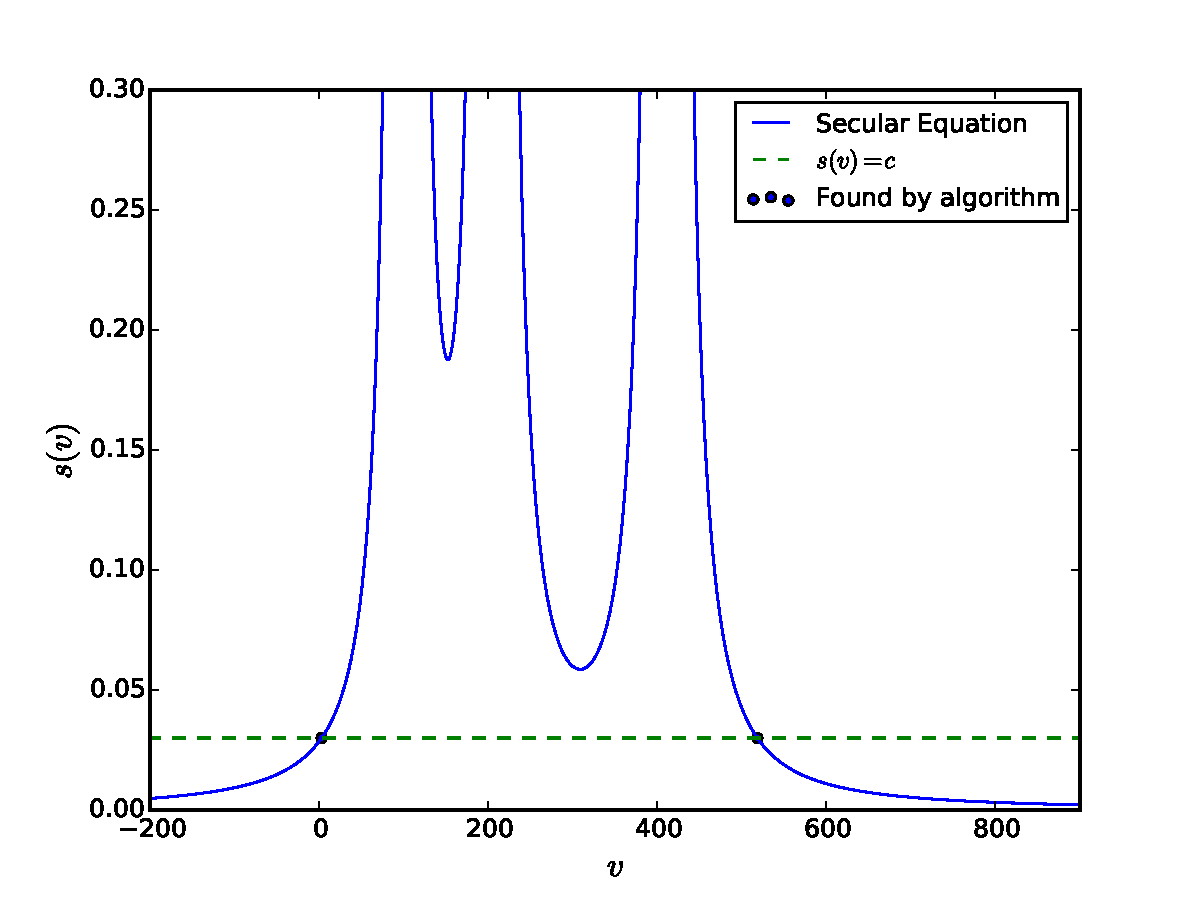
\includegraphics[trim=0in 0in 0.5in 0.5in,clip,width=1\linewidth]{secular}
\caption{Plot of secular equation for a single line in the RTS-96. Note that $s(v)$ approaches infinity at the three poles, and there could be as many as six solutions if $c$ were large enough.}
\label{fig:secular}
\end{figure}

%\begin{figure}
%\centering
%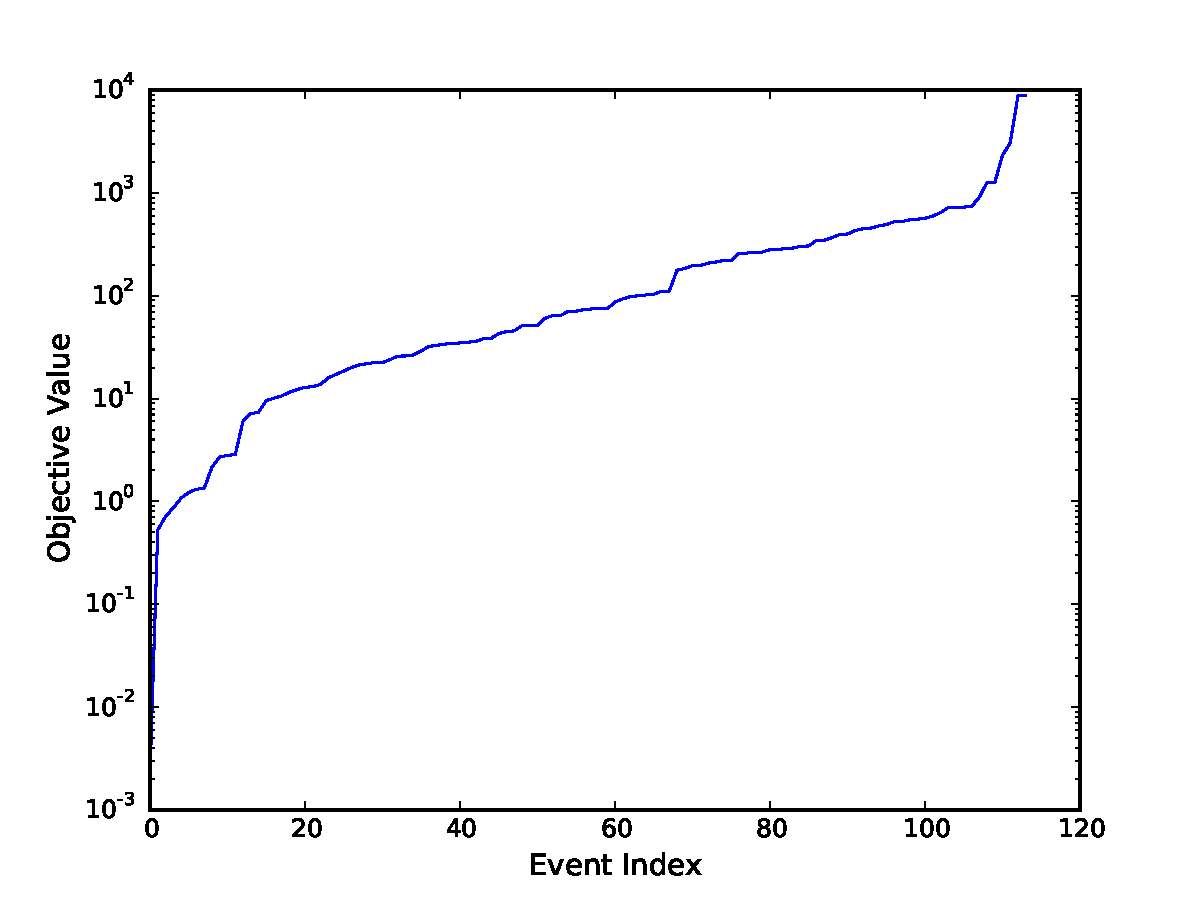
\includegraphics[width=1\linewidth]{../images/scores}
%\caption{Semilogarithmic plot of sorted objective values for RTS-96 temporal instanton analysis. (Note that six lines are missing objective values. The algorithm did not produce solutions for these lines due to numerical instability.)}
%\label{fig:scores}
%\end{figure}

\begin{figure}[t]
\centering
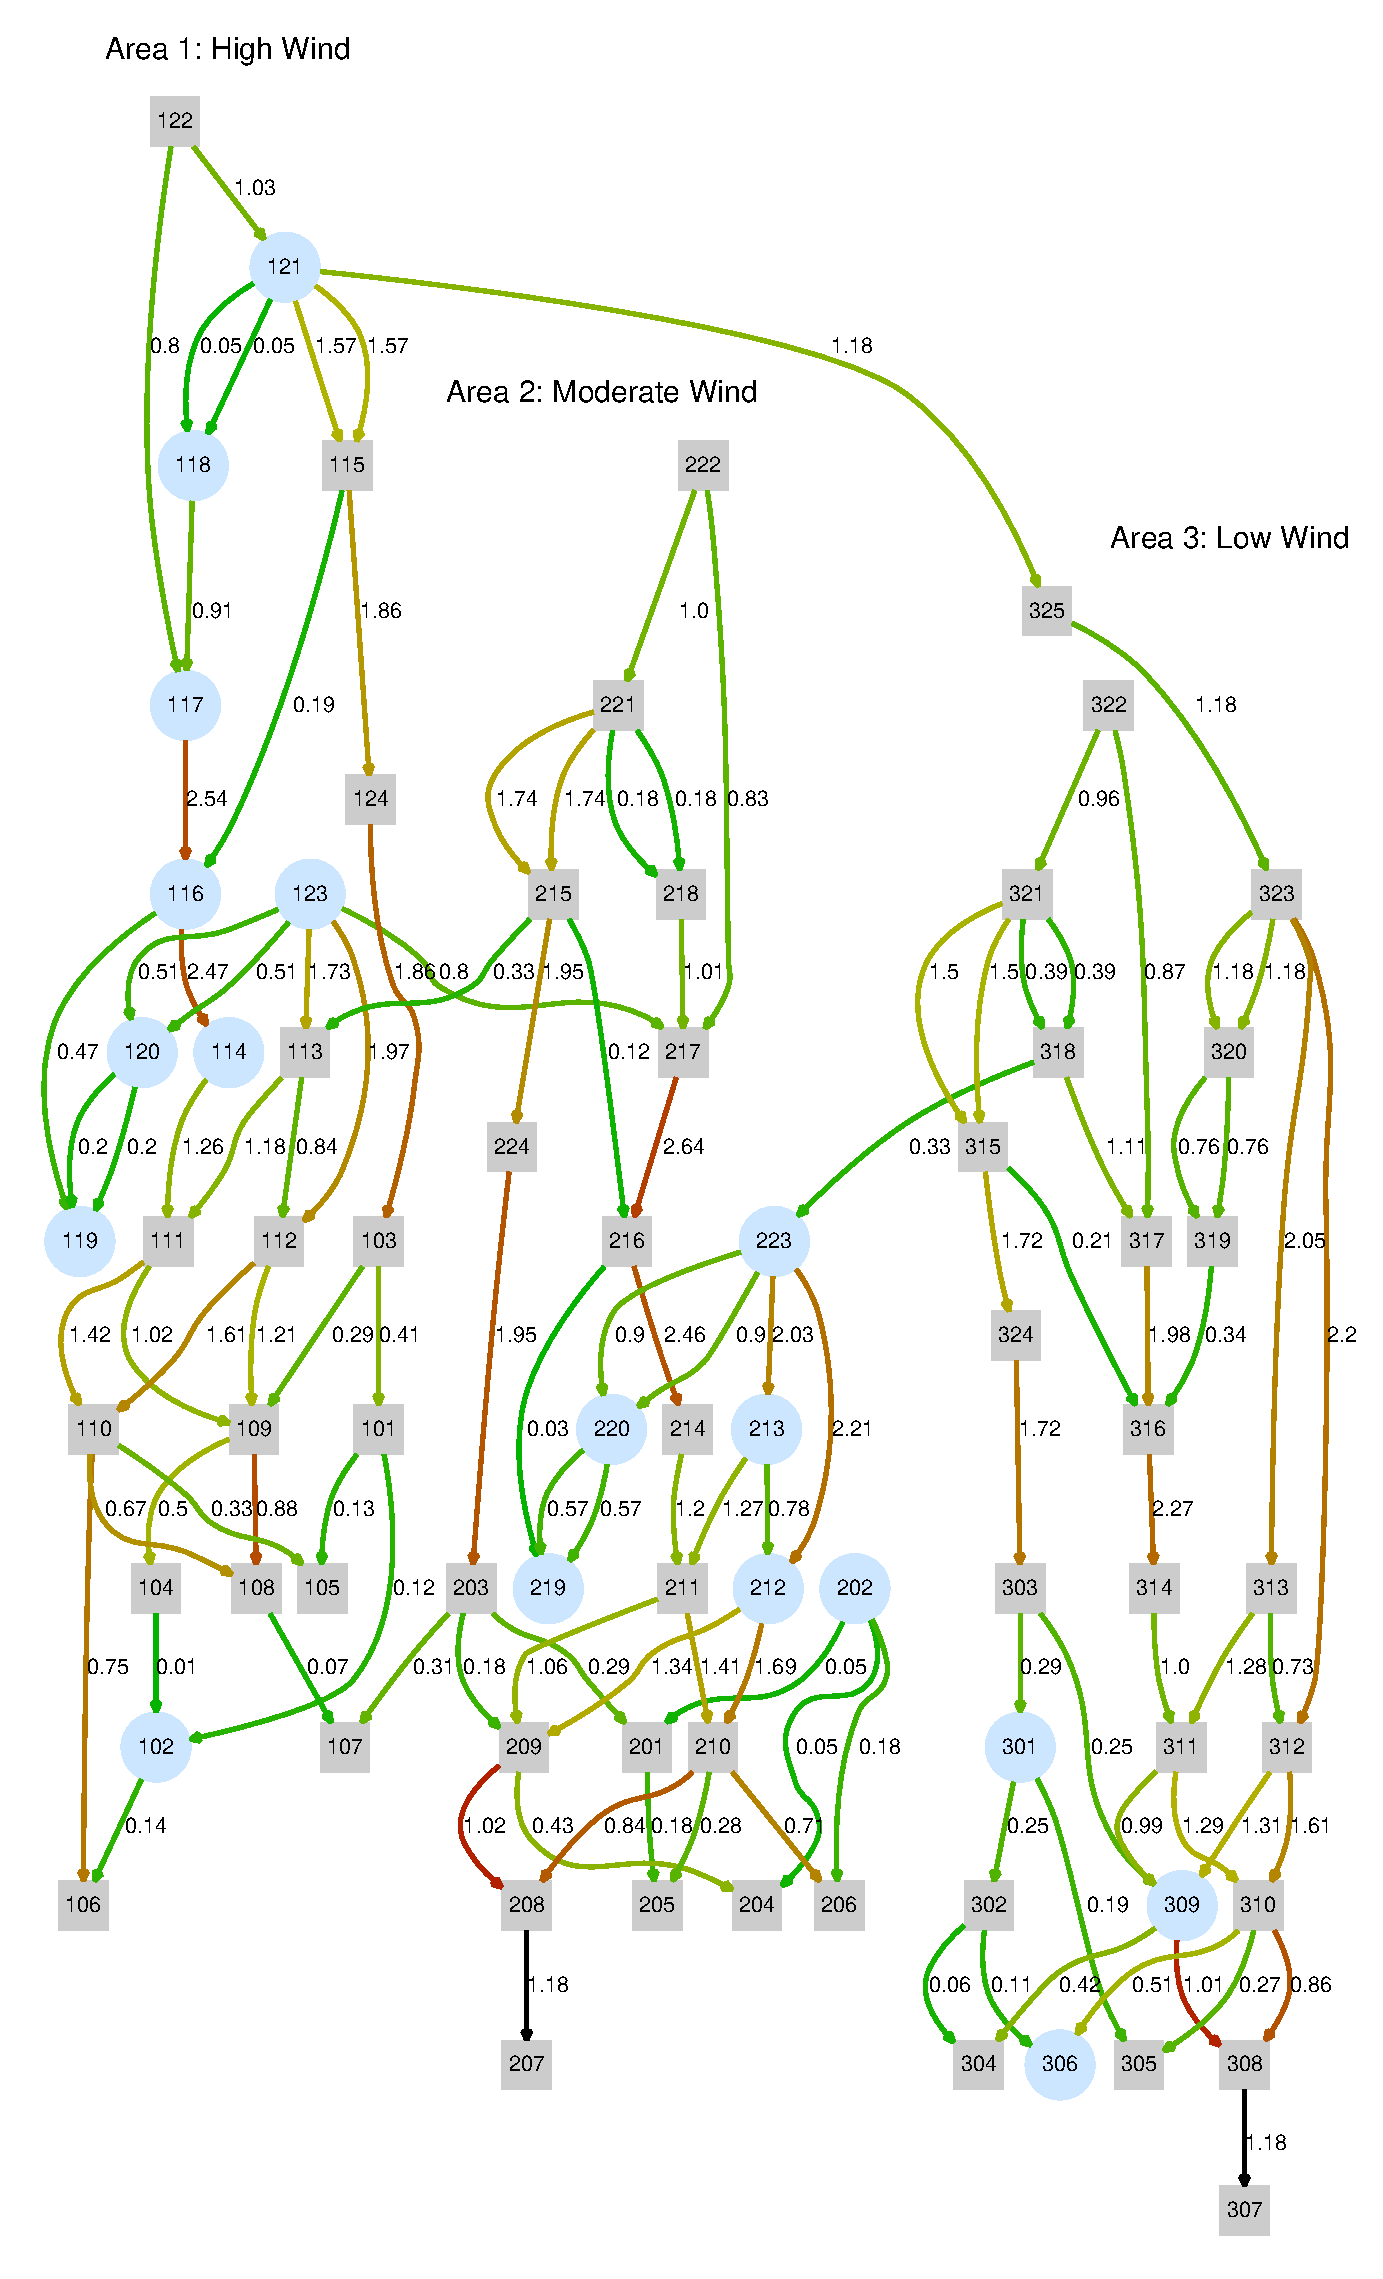
\includegraphics[width=1\linewidth]{line118}
\caption{Graph depiction of RTS-96 system state under instanton conditions at time step 2 of 3. The stressed line is between buses 121 and 325 (top center). wind-farms are indicated by blue, and lines are colored according to how close their flows are to static active power limits.}
\label{fig:line118}
\end{figure}

\section{Conclusions}

The paper has extended instanton analysis to consider the temperature
dynamics of overloaded lines. The resulting formulation is a
quadratically constrained quadratic program (QCQP)\@. A
computationally cheap algorithm has been developed for obtaining
candidate solutions of this QCQP\@.  There is a great deal of
flexibility in the temporal instanton model that has yet to be
explored. In future work we plan to include transformers, consider the
effects of ambient conditions in greater detail, and test the limits
of the algorithm using larger networks with many time steps.


% The paper will close with a discussion of how other
%components, such as voltage regulators, may affect the formulation.

%\section*{Acknowledgment}

%\section*{References}

% can use a bibliography generated by  as a .bbl file
% BibTeX documentation can be easily obtained at:
% http://www.ctan.org/tex-archive/biblio/bibtex/contrib/doc/
% The IEEEtran BibTeX style support page is at:
% http://www.michaelshell.org/tex/ieeetran/bibtex/
\bibliographystyle{IEEEtran}
% argument is your BibTeX string definitions and bibliography database(s)
%\bibliography{IEEEabrv,../bib/paper}
\bibliography{powerTechBib}

\end{document}


